\documentclass[10pt,conference]{IEEEtran}
\usepackage{cite}
\usepackage[pdftex]{graphicx}
\graphicspath{{figs/}}
\DeclareGraphicsExtensions{.pdf,.png,.jpeg,.jpg}
\usepackage[cmex10]{amsmath}
\usepackage{amssymb}
\interdisplaylinepenalty=2500
\usepackage{array}
\usepackage{url}
\usepackage{booktabs}
\usepackage{placeins}
\usepackage[caption=false,font=footnotesize]{subfig}

\newif\iffinal
\finalfalse
\newcommand{\cmtid}{118}

\title{Deep Learning-Based Acne Severity Classification Across Facial Regions with a Mobile Teledermatology Prototype}

\iffinal
\author{
\IEEEauthorblockN{Lucas Gonzaga Andrade}
\IEEEauthorblockA{Federal Institute of Education, Science and Technology of Cear\'a (IFCE)\\
Fortaleza, CE, Brazil}
\and
\IEEEauthorblockN{Roger Moura Sarmento}
\IEEEauthorblockA{Federal Institute of Education, Science and Technology of Cear\'a (IFCE)\\
Fortaleza, CE, Brazil}
}
\else
\author{SIBGRAPI Paper ID: \cmtid \\ }
\fi

\begin{document}
\maketitle

\begin{abstract}
Acne vulgaris is a highly prevalent inflammatory skin disease whose severity assessment remains subjective and specialist-dependent, limiting access in teledermatology scenarios. This paper presents a Region-Aware ResNet-18 for automatic four-level facial acne severity classification from region crops. Anatomical context is encoded through learnable region embeddings fused with visual features extracted by a shared ResNet-18 backbone. Facial regions are obtained with YOLOv8 and resized to $224\times224$. The model was trained on a combined Acne04/Acne Level dataset with augmentation and class-weighted cross-entropy. On 1{,}090 held-out test crops, the system achieved 95.2\% accuracy and weighted F1-score of 0.95, with regional weighted F1 $\geq$ 0.93. Thirty perturbation runs yielded mean accuracy of 93.3\% ($\sigma=0.46\%$). A Flutter prototype illustrates the intended mobile workflow, although on-device inference was not yet deployed.
\end{abstract}

\begin{IEEEkeywords}
acne severity classification, convolutional neural networks, ResNet, computer vision, teledermatology, clinical decision support
\end{IEEEkeywords}

\section{Introduction}
Acne vulgaris is a chronic inflammatory disease of the pilosebaceous unit that affects a large share of adolescents and adults, producing physical sequelae and psychosocial impact \cite{zaenglein2018acne,samuels2020acne,vallerand2018risk}. Clinical grading depends on visual inspection and is sensitive to inter-observer variability, illumination, and specialist availability \cite{hayashi2008grading}. In parallel, teledermatology has expanded remote dermatological care through smartphone imaging \cite{moreno2017teledermatology,tran2011mobile}, creating demand for standardized, reproducible, and lightweight automated assessment tools.

Most prior acne systems rely on multi-stage pipelines: lesion detection followed by counting or severity estimation. Although effective in controlled settings, these approaches increase annotation cost, computational complexity, and error propagation between stages. Direct severity classifiers simplify inference but often ignore that acne distribution and appearance vary across facial regions. Vision Transformers and hybrid CNN--Transformer models improve representation capacity, yet their computational cost limits mobile deployment.

This work proposes a unified Region-Aware ResNet-18 that classifies severity directly from facial-region crops. A learnable embedding injects anatomical identity into a single shared backbone, avoiding multiple specialized networks. Our contributions are:
\begin{itemize}
\item a lightweight region-aware ResNet-18 with 64-dimensional region embeddings;
\item a YOLOv8-based preprocessing pipeline for five facial regions;
\item a broad evaluation protocol covering global, class-wise, regional, stability, and confidence analyses;
\item a Flutter teledermatology prototype demonstrating the intended deployment workflow.
\end{itemize}

Unlike lesion-centric methods, we perform four-level severity classification from region crops, preserving anatomical context while keeping the pipeline suitable for mobile health applications.

\section{Related Work}
CNNs have achieved strong performance in dermatological image analysis, including melanoma detection and general lesion classification \cite{nasr2016melanoma,brinker2019cnn}. For acne, prior work includes Faster R-CNN/YOLO-based lesion detectors combined with grading modules \cite{huynh2022automatic}, unified grading frameworks \cite{lin2022kieglfn}, and ensemble CNN classifiers \cite{liu2022acnegrader,shen2018acne,wu2019joint}. ResNet architectures remain attractive because they balance accuracy, training stability, and deployment cost \cite{he2016resnet}.

However, many studies report only global metrics and overlook regional consistency, run-to-run stability, and confidence behavior---aspects that matter for clinical decision support. Motivated by these gaps, we evaluate the proposed model beyond headline accuracy and connect it to a mobile teledermatology workflow \cite{byamba2015mobile}.

\section{Proposed Method}
\subsection{Dataset and Preprocessing}
We combined two public corpora widely used in acne research: Acne04 (\texttt{acne\_1024}, 1{,}406 frontal-face images) and Acne Level (\texttt{Dataset/}, 1{,}457 images organized by severity folders). Both follow four Hayashi-aligned severity levels (0--3). Although both target acne severity classification, they differ in organization, illumination, and patient appearance, which increases evaluation difficulty and better reflects heterogeneous acquisition conditions. Representative samples from both sources, together with the five facial zones used by the classifier---forehead, left cheek, right cheek, nose, and chin---are shown in Figure~\ref{fig:datasets}.

\begin{figure}[!htbp]
\centering
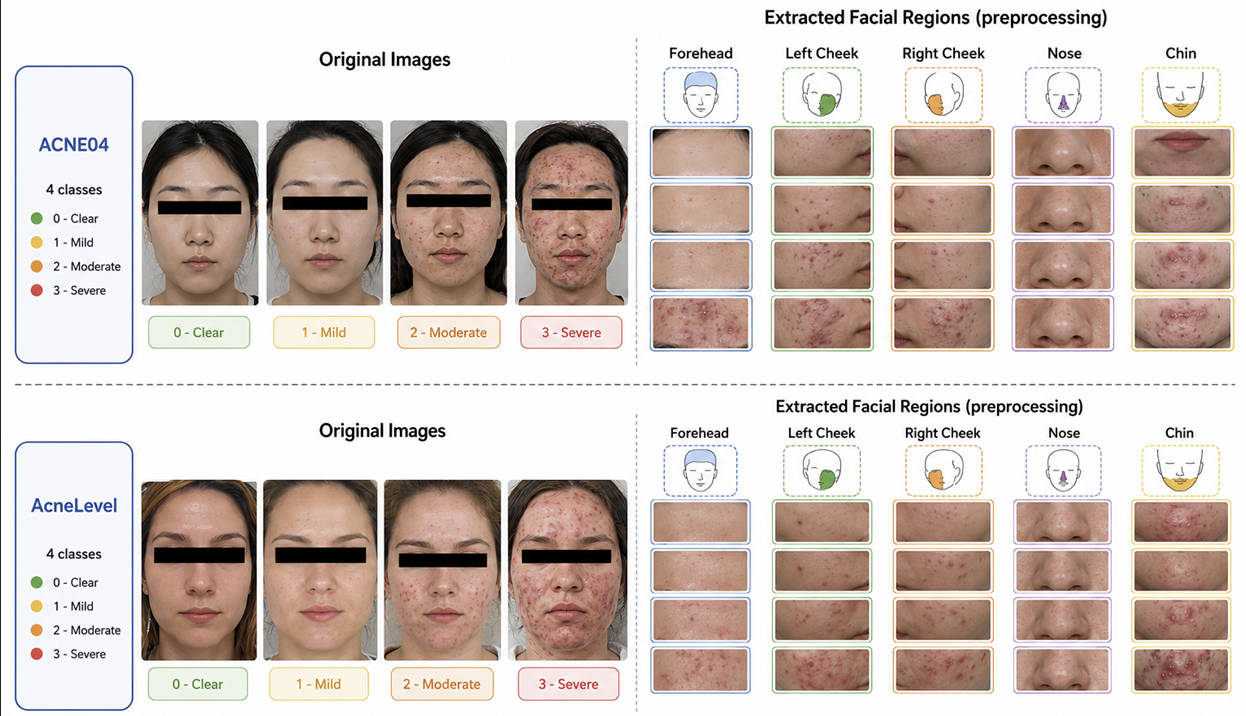
\includegraphics[width=0.88\columnwidth]{fig2_datasets.jpg}
\caption{Representative Acne04 and Acne Level samples with extracted facial regions used in preprocessing.}
\label{fig:datasets}
\end{figure}
\FloatBarrier

After consolidation, images were processed with a custom YOLOv8 detector trained to localize the five anatomical regions. Each detected crop was resized to $224\times224$ pixels and normalized consistently with training. The final split was 70\% train, 15\% validation, and 15\% test, preserving independence between training and evaluation samples. This preprocessing stage converts heterogeneous full-face photographs into standardized region-level inputs suitable for the shared classifier.

\subsection{System Pipeline}
The end-to-end workflow comprises five stages: image acquisition, YOLOv8-based region extraction, Region-Aware ResNet-18 inference, four-level severity prediction, and mobile visualization in the teledermatology prototype. As summarized in Figure~\ref{fig:pipeline}, the design keeps acquisition on the smartphone while concentrating computational effort on compact region crops rather than full-resolution portraits.

\begin{figure}[!htbp]
\centering
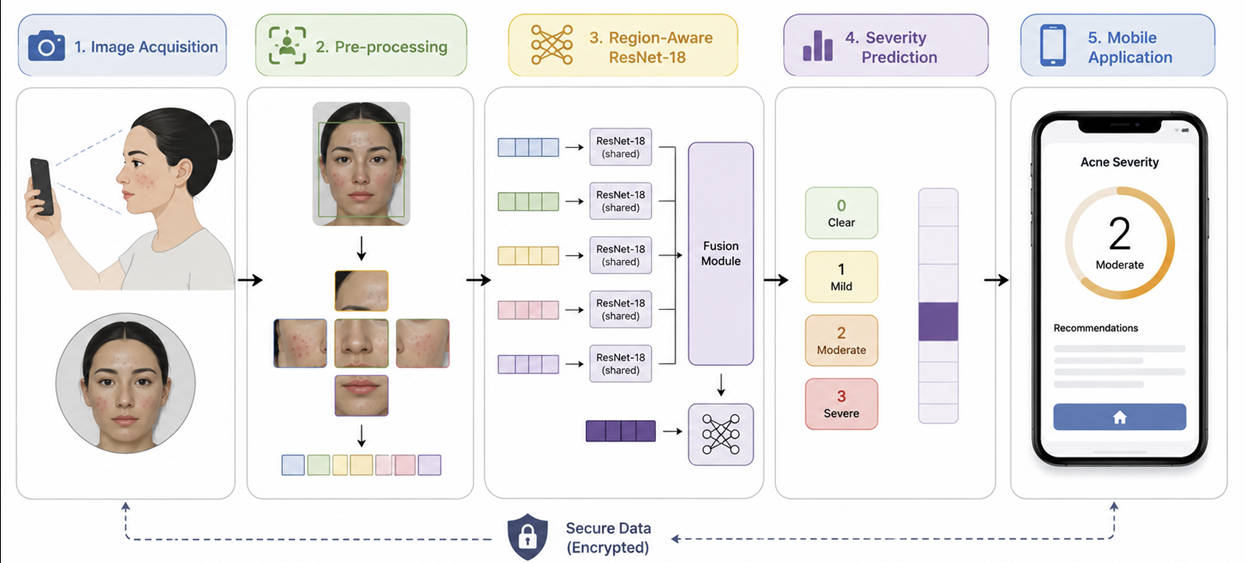
\includegraphics[width=0.88\columnwidth]{fig1_pipeline.jpg}
\caption{Overview of the proposed pipeline from acquisition to mobile reporting.}
\label{fig:pipeline}
\end{figure}
\FloatBarrier

Separating detection from classification reduces error propagation and allows each module to be updated independently. Region crops also align the inference input with the labels available in the training corpora, which are defined at the zone level rather than for the entire face.

\subsection{Region-Aware ResNet-18}
The proposed architecture enriches visual features with explicit anatomical context. Each region crop is processed by a ResNet-18 backbone trained from scratch; after global average pooling, the visual descriptor $\mathbf{f}\in\mathbb{R}^{512}$ is concatenated with a learnable region embedding $\mathbf{e}_r\in\mathbb{R}^{64}$, as depicted in Figure~\ref{fig:arch}:
\begin{equation}
\mathbf{z} = [\mathbf{f}\,\|\,\mathbf{e}_r] \in \mathbb{R}^{576}.
\end{equation}
The fused vector is passed to a classifier composed of fully connected layers with batch normalization, ReLU, and dropout, producing four severity logits. This design allows one shared backbone to adapt its decision boundary according to the input region without training separate models per zone.

\begin{figure}[!htbp]
\centering
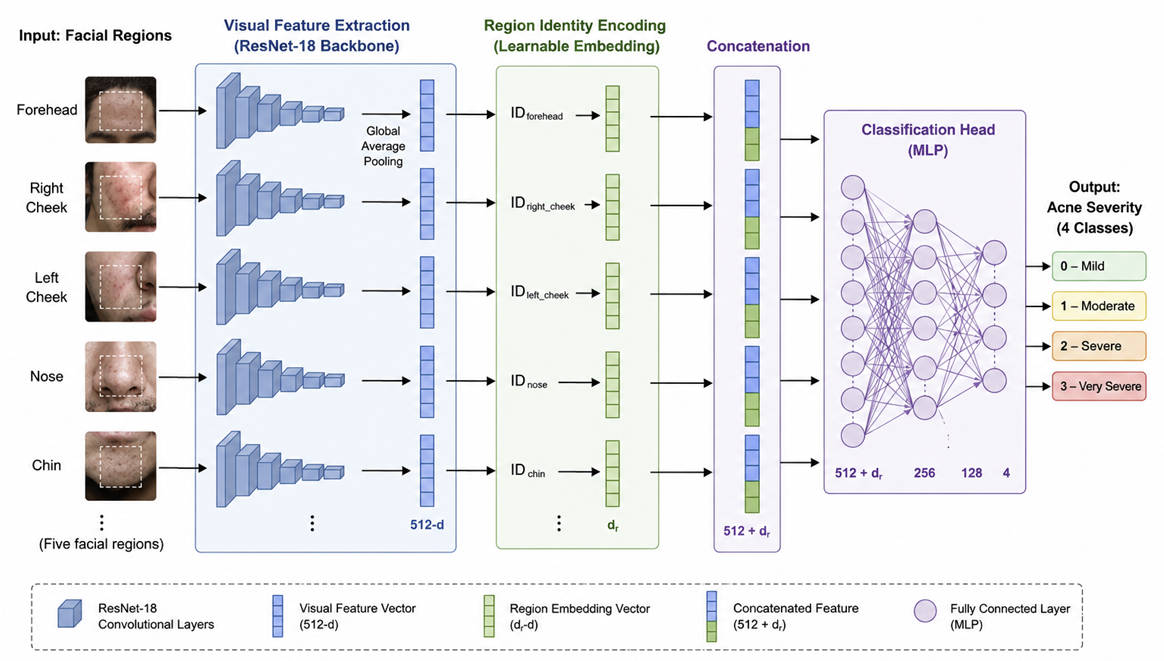
\includegraphics[width=0.88\columnwidth]{fig3_architecture.jpg}
\caption{Region-Aware ResNet-18 architecture with learnable region embeddings fused before classification.}
\label{fig:arch}
\end{figure}
\FloatBarrier

Compared with multi-network or attention-heavy alternatives, the embedding layer adds only a small number of parameters while preserving low inference cost, which is important for smartphone-based teledermatology.

\subsection{Training Protocol}
Training was conducted in PyTorch with Adam ($\text{lr}=10^{-4}$), weighted cross-entropy loss, batch size 16, and up to 40 epochs. Class weights mitigated imbalance among severity levels. We applied ReduceLROnPlateau scheduling and early stopping based on robust validation behavior. Augmentations included horizontal flip ($p=0.5$), rotation ($\pm25^\circ$), color jitter, Gaussian blur, and random erasing. Train and validation splits were merged for the final model selection criterion.

\subsection{Evaluation Protocol}
We report accuracy, precision, recall, and F1-score globally and per class. Regional weighted metrics assess whether anatomical context improves consistency across zones. Stability was measured with 30 independent test runs under mild perturbations compatible with smartphone capture variability. Confidence analysis examined softmax score distributions for correct and incorrect predictions. This three-view protocol---class discrimination, regional consistency, and operational robustness---reduces overinterpretation of a single favorable metric.

\section{Experimental Results}
\subsection{Overall Classification Performance}
The test set contains 1{,}090 region crops. Table~\ref{tab:class} summarizes global performance. The model reached 95.2\% accuracy and weighted F1-score of 0.95. Precision, recall, and F1 remain close across classes, indicating balanced learning despite uneven class frequencies. Grades 0 and 3 achieved the strongest results, whereas grade 2 was the most challenging due to visual overlap with adjacent severities.

\begin{table}[t]
\caption{Per-class classification metrics on the test set}
\label{tab:class}
\centering
\small
\begin{tabular}{lcccc}
\toprule
Grade & Prec. & Rec. & F1 & Sup. \\
\midrule
0 & 0.96 & 0.95 & 0.95 & 318 \\
1 & 0.94 & 0.94 & 0.94 & 412 \\
2 & 0.88 & 0.92 & 0.90 & 110 \\
3 & 1.00 & 1.00 & 1.00 & 250 \\
\midrule
W. avg. & 0.95 & 0.95 & 0.95 & 1090 \\
\bottomrule
\end{tabular}
\end{table}

Most errors occur between neighboring classes, especially between grades 1 and 2, whereas confusion between distant classes (0 and 3) is negligible. This pattern mirrors clinical ambiguity in borderline cases and is confirmed by the confusion matrix in Figure~\ref{fig:conf}, reported in both absolute counts and normalized percentages.

\begin{figure}[!htbp]
\centering
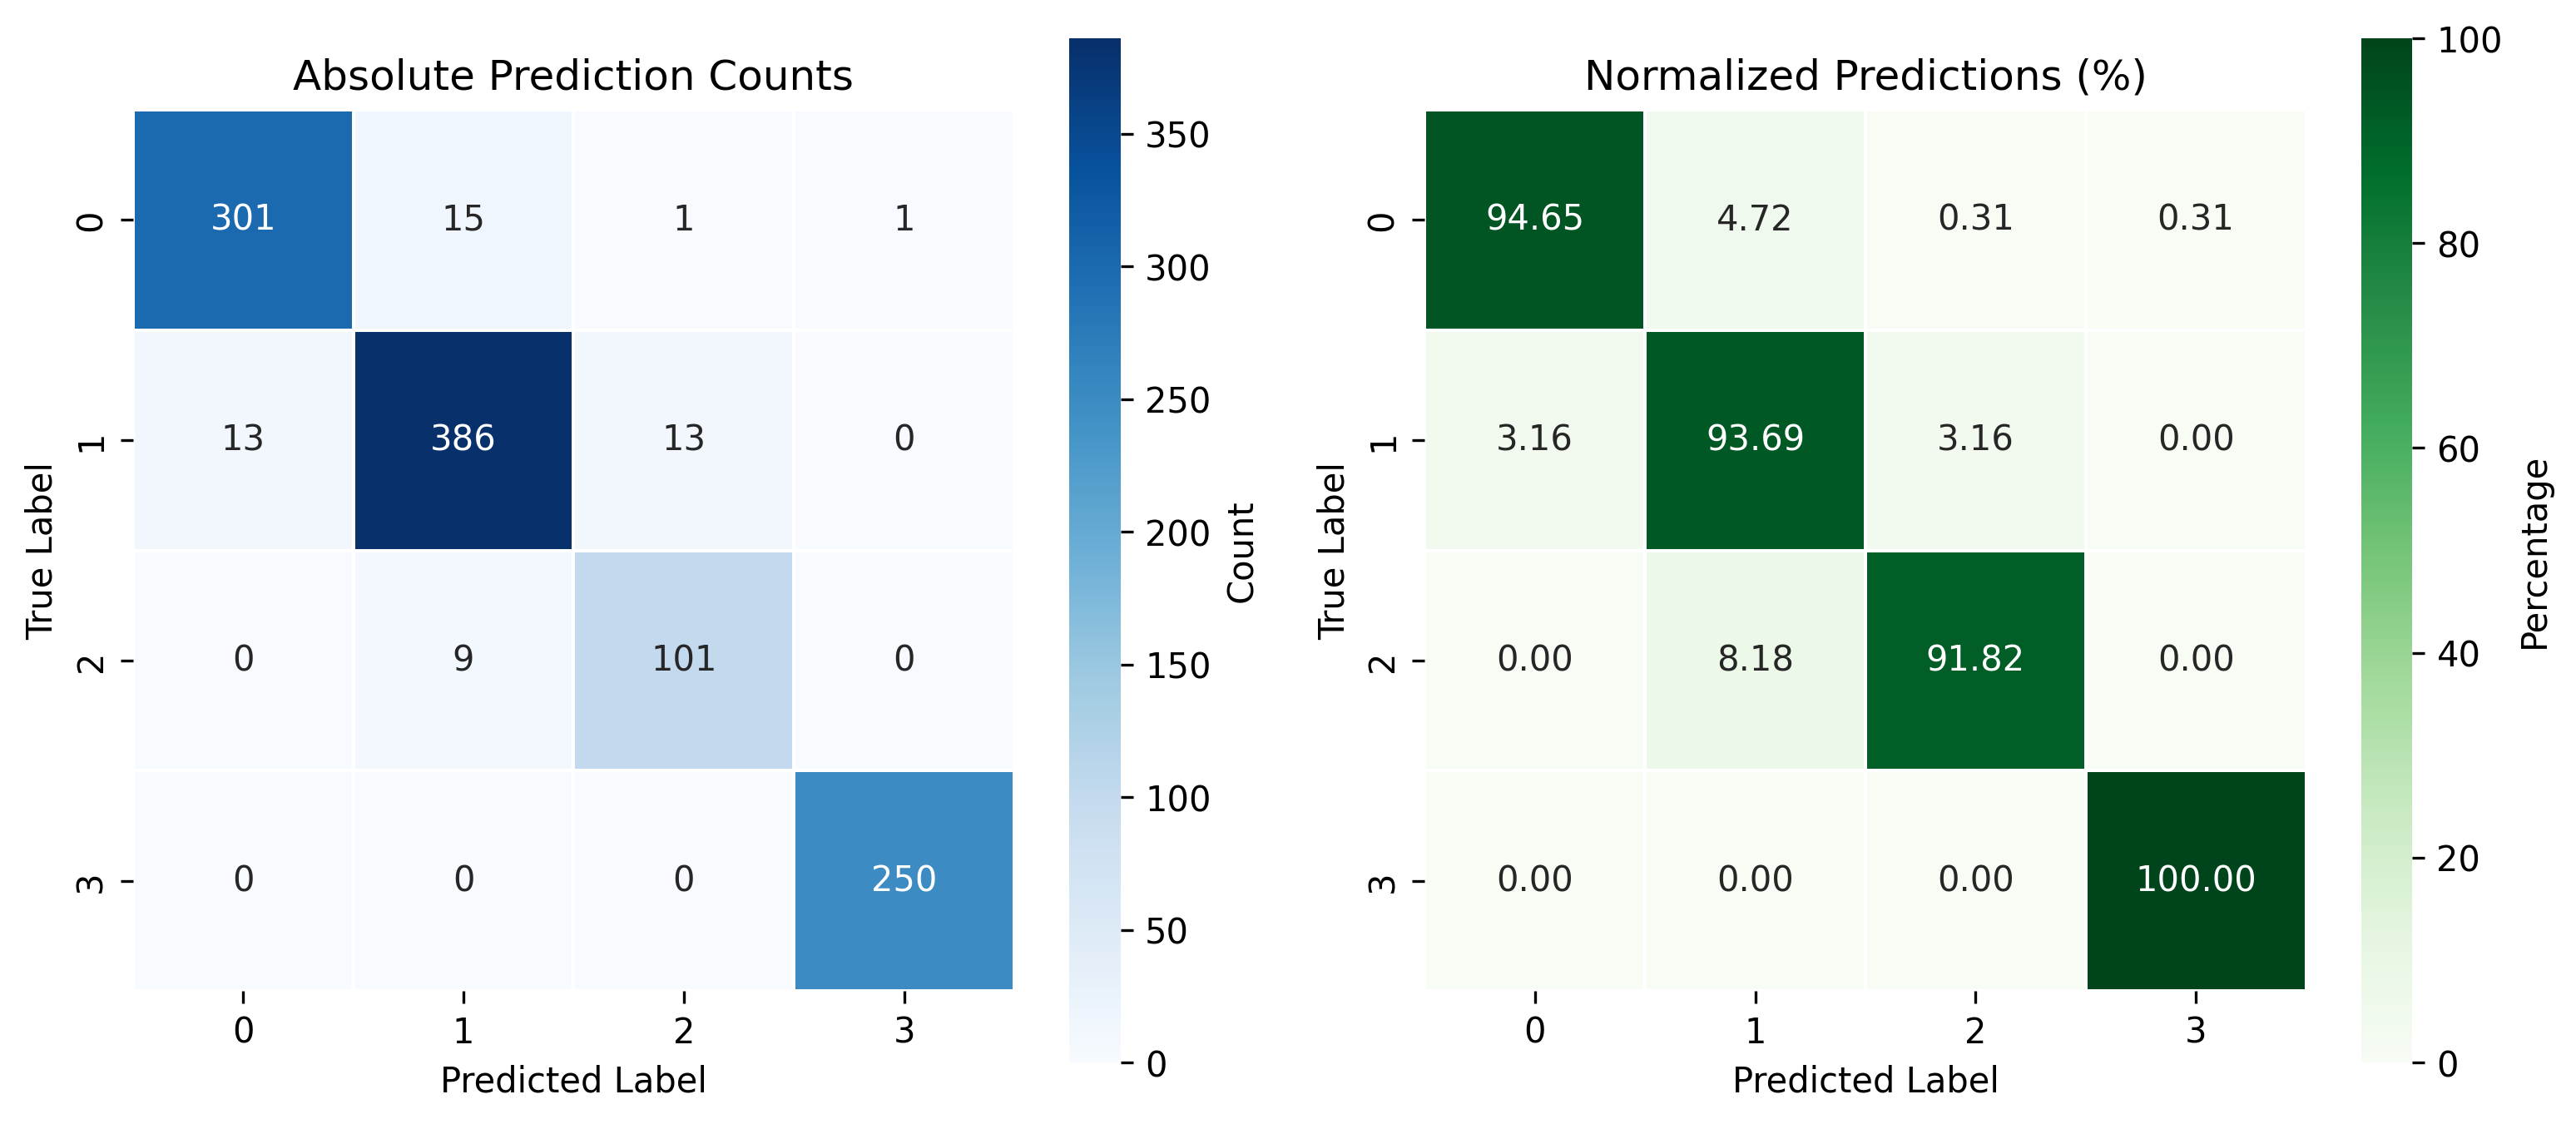
\includegraphics[width=0.88\columnwidth]{fig4_confusion_en.png}
\caption{Confusion matrix on the test set: absolute counts (left) and normalized percentages (right).}
\label{fig:conf}
\end{figure}
\FloatBarrier

The diagonal dominance across all grades indicates systematic rather than random failure modes, with residual errors concentrated where severity boundaries are inherently subjective.

\subsection{Regional Performance Analysis}
Because region identity is explicitly encoded, we analyzed whether performance remains stable across facial zones. Table~\ref{tab:regions} reports weighted metrics by region. All regions achieved F1 $\geq$ 0.93. Forehead obtained the best result (F1 = 0.99), while chin and left cheek were comparatively harder yet still strong (F1 = 0.93). Lower cheek/chin performance may reflect texture variability, facial hair, shadows, and less homogeneous lesion distribution---factors commonly observed in mobile image acquisition.

\begin{table}[t]
\caption{Weighted performance by facial region}
\label{tab:regions}
\centering
\small
\begin{tabular}{lcccc}
\toprule
Region & Prec. & Rec. & F1 & Sup. \\
\midrule
Forehead & 0.99 & 0.99 & 0.99 & 93 \\
Chin & 0.94 & 0.93 & 0.93 & 329 \\
Nose & 0.97 & 0.97 & 0.97 & 103 \\
L. cheek & 0.94 & 0.93 & 0.93 & 169 \\
R. cheek & 0.96 & 0.96 & 0.96 & 396 \\
\bottomrule
\end{tabular}
\end{table}

These results support the main architectural claim: a single ResNet-18 with region embeddings can learn zone-specific behavior without maintaining five independent models.

\subsection{Robustness and Confidence Analysis}
To assess sensitivity to realistic capture variability, we repeated inference on the test set across 30 independent runs with light input perturbations. Mean accuracy was 93.3\% with $\sigma=0.46\%$, indicating low run-to-run variability under conditions compatible with smartphone photography. The corresponding accuracy distribution is shown in Figure~\ref{fig:stability} and, together with the adjacent-class confusion patterns in Figure~\ref{fig:conf}, supports operational stability despite minor pose or illumination changes.

\begin{figure}[!htbp]
\centering
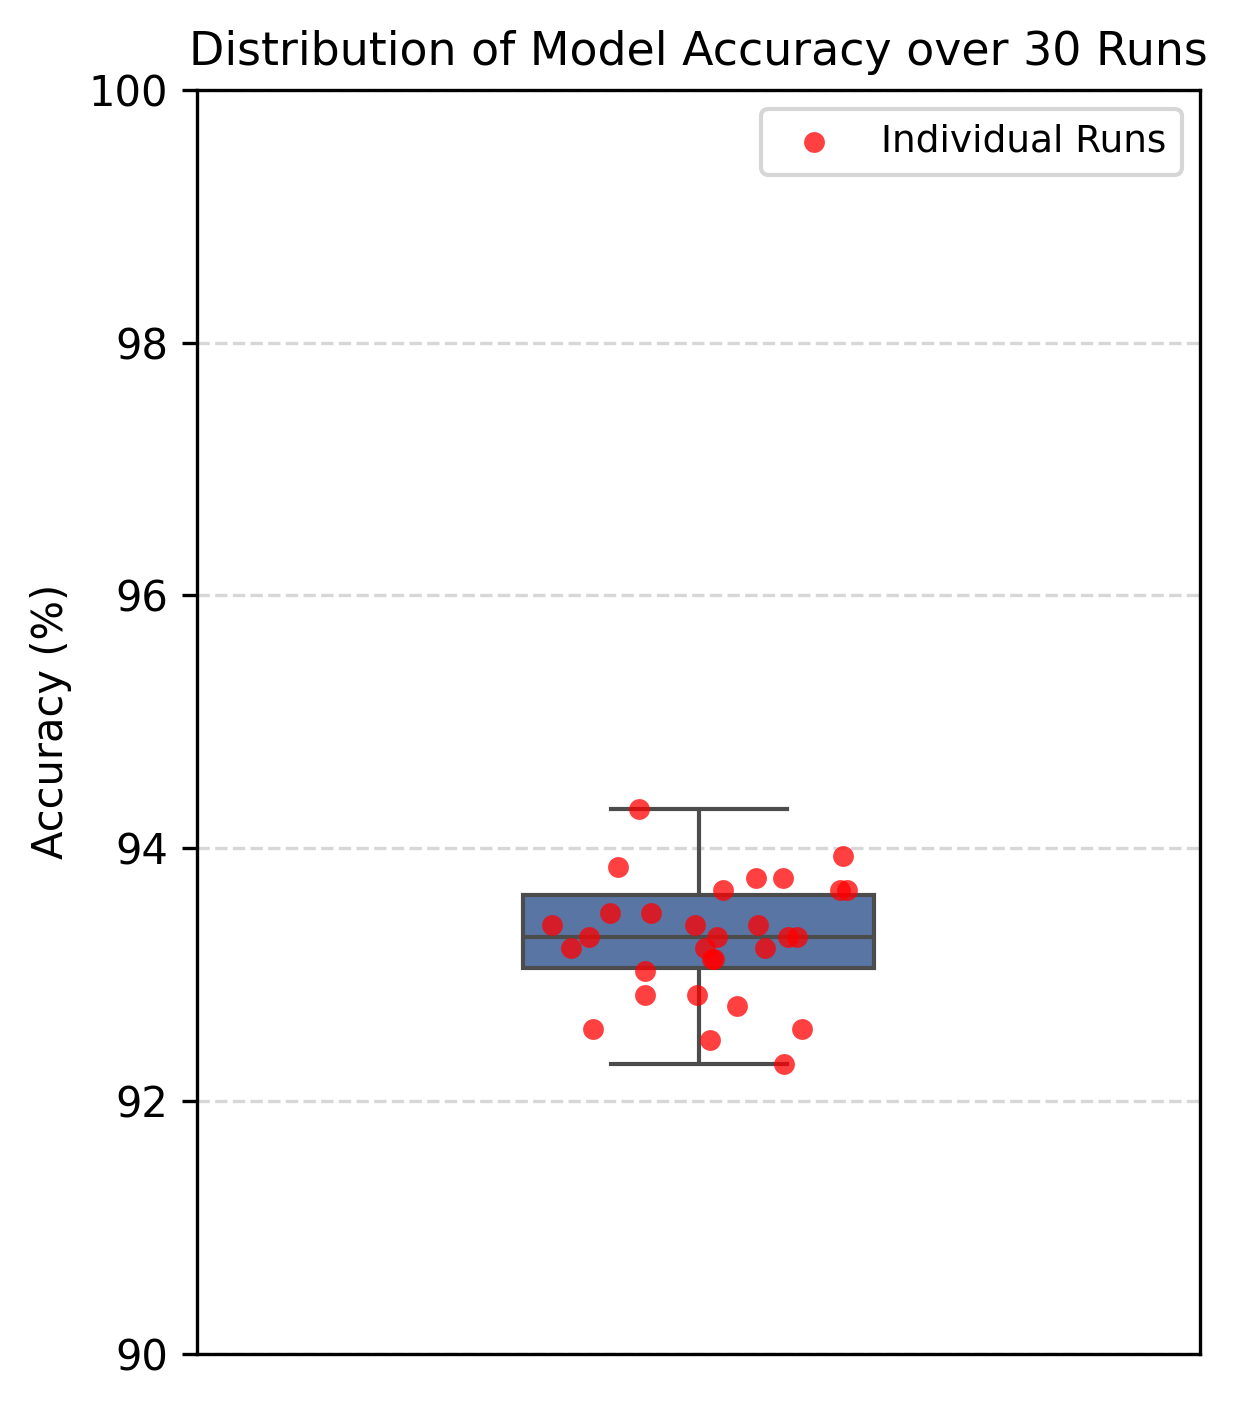
\includegraphics[width=0.70\columnwidth]{fig5_stability_en.png}
\caption{Accuracy distribution over 30 independent robustness evaluations.}
\label{fig:stability}
\end{figure}
\FloatBarrier

Confidence analysis showed that correct predictions usually received very high softmax scores, while a subset of incorrect predictions was also overconfident. Therefore, calibration techniques and selective referral policies are recommended before clinical deployment, especially for borderline cases between grades 1 and 2.

\section{Mobile Prototype}
To demonstrate practical integration, we developed a Flutter teledermatology prototype supporting login, guided image submission, remote inference, and longitudinal tracking. The interface covers the main stages of the intended workflow---home, guided capture, region selection, analysis progress, severity result with confidence indicator, and analysis history---as illustrated in Figure~\ref{fig:app}.

\begin{figure}[!htbp]
\centering
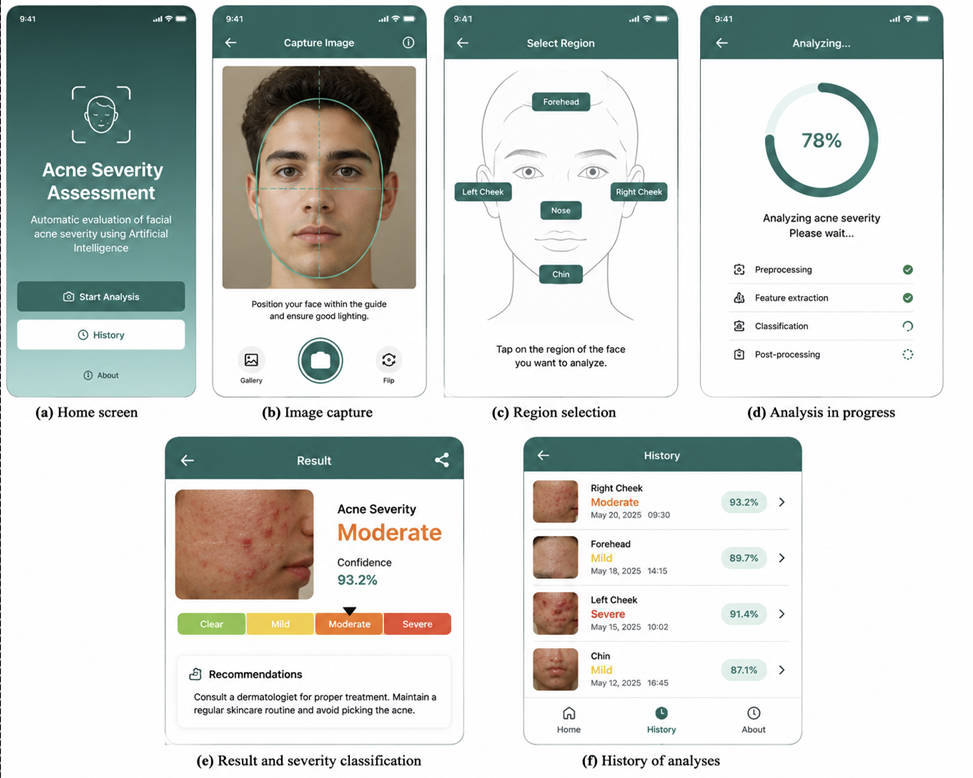
\includegraphics[width=0.88\columnwidth]{fig6_app.jpg}
\caption{Mobile teledermatology prototype screens for capture, analysis, and history.}
\label{fig:app}
\end{figure}
\FloatBarrier

At the time of writing, on-device inference is not yet integrated; the application demonstrates interface and workflow design rather than validated clinical deployment. Separating the mobile client from the inference service facilitates future model updates and uncertainty-based triage rules.

\section{Discussion}
The experimental results show that explicit anatomical encoding provides a simple and effective way to enrich a lightweight CNN without multi-stage lesion pipelines. The unified backbone reduces parameter redundancy and simplifies maintenance relative to one-model-per-region strategies. Strong global metrics combined with stable regional performance suggest that the method is suitable as a decision-support tool for remote monitoring.

From a deployment perspective, low variance across runs (Figure~\ref{fig:stability}) indicates operational reliability, whereas the adjacent-class confusion visible in Figure~\ref{fig:conf} reflects clinically plausible ambiguity. A hybrid policy---automatic triage for high-confidence non-borderline cases and specialist review for uncertain ones---aligns model strengths with safe clinical use.

\section{Limitations and Conclusion}
This study uses merged public datasets and does not yet cover the full diversity of skin phototypes, devices, and real-world lighting. Labels are region-level severity grades rather than lesion-level annotations, and the mobile prototype was not evaluated prospectively in clinical teledermatology.

We presented a Region-Aware ResNet-18 for four-level acne severity classification from facial-region crops, achieving 95.2\% test accuracy with consistent cross-region behavior and low stability variance. Future work includes confidence calibration, external validation, on-device inference, and broader demographic representation. The system is intended as clinical decision support and does not replace professional diagnosis.

\begin{thebibliography}{99}
\bibitem{zaenglein2018acne}
A.~L. Zaenglein, ``Acne vulgaris,'' \emph{New England Journal of Medicine}, vol. 379, no. 14, pp. 1343--1352, 2018.

\bibitem{samuels2020acne}
D.~V. Samuels \emph{et al.}, ``Acne vulgaris and risk of depression and anxiety: a meta-analytic review,'' \emph{J. Amer. Acad. Dermatol.}, vol. 83, no. 2, pp. 532--541, 2020.

\bibitem{vallerand2018risk}
I.~A. Vallerand \emph{et al.}, ``Risk of depression among patients with acne in the UK,'' \emph{Brit. J. Dermatol.}, vol. 178, no. 3, pp. e194--e195, 2018.

\bibitem{hayashi2008grading}
N.~Hayashi \emph{et al.}, ``Development of a new acne severity grading system,'' \emph{J. Dermatol.}, vol. 35, no. 5, pp. 255--260, 2008.

\bibitem{moreno2017teledermatology}
D.~Moreno-Ram{\'i}rez and G.~Argenziano, ``Teledermatology and mobile applications in the management of patients with skin lesions,'' \emph{Acta Dermato-Venereologica}, vol. 97, no. 4, pp. 412--418, 2017.

\bibitem{huynh2022automatic}
Q.~T. Huynh \emph{et al.}, ``Automatic acne object detection and acne severity grading using smartphone images and AI,'' \emph{Diagnostics}, vol. 12, no. 8, 2022.

\bibitem{lin2022kieglfn}
Y.~Lin \emph{et al.}, ``KIEGLFN: A unified acne grading framework on face images,'' \emph{Comput. Methods Programs Biomed.}, vol. 221, 2022.

\bibitem{liu2022acnegrader}
S.~Liu \emph{et al.}, ``AcneGrader: An ensemble pruning of deep learning base models to grade acne,'' \emph{Skin Res. Technol.}, vol. 28, no. 5, pp. 677--688, 2022.

\bibitem{shen2018acne}
X.~Shen \emph{et al.}, ``An automatic diagnosis method of facial acne vulgaris based on CNN,'' \emph{Scientific Reports}, vol. 8, p. 5839, 2018.

\bibitem{wu2019joint}
X.~Wu \emph{et al.}, ``Joint acne image grading and counting via label distribution learning,'' in \emph{Proc. IEEE/CVF ICCV}, 2019, pp. 10642--10651.

\bibitem{nasr2016melanoma}
E.~Nasr-Esfahani \emph{et al.}, ``Melanoma detection by analysis of clinical images using CNN,'' in \emph{Proc. IEEE EMBC}, 2016, pp. 1373--1376.

\bibitem{brinker2019cnn}
T.~J. Brinker \emph{et al.}, ``A CNN trained with dermoscopic images performed on par with 145 dermatologists,'' \emph{Eur. J. Cancer}, vol. 111, pp. 148--154, 2019.

\bibitem{he2016resnet}
K.~He, X.~Zhang, S.~Ren, and J.~Sun, ``Deep residual learning for image recognition,'' in \emph{Proc. IEEE CVPR}, 2016, pp. 770--778.

\bibitem{byamba2015mobile}
K.~Byamba \emph{et al.}, ``Mobile teledermatology for a prompter and more efficient dermatological care in rural Mongolia,'' \emph{Brit. J. Dermatol.}, vol. 173, no. 1, pp. 265--267, 2015.

\bibitem{tran2011mobile}
K.~Tran \emph{et al.}, ``Mobile teledermatology in the developing world,'' \emph{J. Amer. Acad. Dermatol.}, vol. 64, no. 2, pp. 302--309, 2011.
\end{thebibliography}

\end{document}
